

\section{Bussysteme}

\subsection{CAN-Bus}
    \subsubsection{Anwendung}
    Entwickelt von der Robert Bosch GmbH 1985, ist der CAN-Bus (Controller Area Network) 
    das erste in Serie eingeführte Bussystem. Hauptanwendungsgebiet ist der
    Nachrichtentransfer zwischen Steuergeräten, Sensoren und Aktoren in 
    einem System mit Echtzeitgesteuerten Anwendungen.~\cite{LA_CAN1}

    Unter den Echtzeitgesteuerten Anwendungsgebieten befinden sich beispielhaft:
    \begin{description}
    \item[-] Steuerung der Kombiinstrument
    \item[-] Fahrassistenzsysteme(ABS, ESP, etc.)
    \item[-] Motormanagement
    \item[-] Getriebesteuerung
    \end{description}
    1992 wurde CAN, mit der Mercedes S-Klasse, erstmals der Öffentlichkeit zugänglich gemacht. 
    Seit 1995 ist CAN das am meisten verbreitete Bussystem in Automobilanwendungen.
 
    CAN zeichnet sich durch eine simple, effiziente und robuste Datenübertragung für Netzwerke in 
    Fahrzeugen aus. Mit der stetig ansteigenden Anzahl an Steuergeräten, und der steigenden 
    Schwierigkeit diese zu verbinden setzte sich CAN schnell als simple und effektive 
    Lösung durch, Steuergeräte kosteneffizient zu verbinden.~\cite{LA_CAN2}

    \subsubsection{Topologie}
    Der CAN-Standard sieht vor, dass kein zentrales Steuerungselement benötigt wird.
    Am effektivsten wird dieses Designkonzept durch eine Bustopologie unterstützt. Bei diesem
    ist jeder Busteilnehmer direkt mit dem Bus verbunden und kann informationen von jedem anderen
    Teilnehmer empfangen. Aufgrunddessen ist die Bustopologie das am häufigsten gewählte Konzept.
    ~\cite{LA_Bosch_6te_auflage}
    
    \subsubsection{Realisierung}
    Über die Jahre erweiterte sich der Anwendungsbereich von CAN auf Systeme
    die keine Echtzeitfähigkeit benötigen. Darunter fallen die Fahrzeugdiagnose und diverse 
    Komfortsysteme. Konsequenterweise wurde CAN in 2 Klassen unterteilt (CAN B/Lowspeed-CAN, 
    CAN C/Highspeed-CAN), die sich hauptsächlich in ihrer Übertragungsgeschwindigkeit 
    unterscheiden, jedoch auf demselben Standard, der ISO-Norm 11898, basieren und dasselbe 
    Protokoll nutzen. Im Folgenden werden die Unterschiede dieser Klassen erläutert, gefolgt von 
    einigen Anwendungsbeispielen.
    \begin{itemize}
        \item{CAN B / Lowspeed-CAN:}\\
        Über den Lowspeed-CAN-Bus kommunizieren Steuergeräte die für das steuern von 
        Komfortsystemen verantwortlich sind. Dieser weißt daher nur eine maximale 
        Übertragungsgeschwindigkeit von 125kBit/s auf. Einige der simplen Anwendungsgebiete wurden
        von dem später eingeführten LIN-Bus übernommen, jedoch gibt es Anwendungsgebiete die 
        die höhere Datenrate, Fehlertoleranz und Echtzeitfähigkeit fordern, weshalb Lowspeed-CAN immer 
        noch Anwendung findet.
        Es wird zusätzlich meist als Backbone Netzwerk eines LIN-Bus verwendet.
        ~\cite{LA_Bosch_6te_auflage}
        \item{CAN C / Highspeed-CAN:}\\
        Über den Highspeed-CAN kommunizieren Steuergeräte die, aufgrund von schnellen Abläufen, in 
        Ihren Anwendungsgebieten, eine höhere Übertragungsgeschwindigkeit benötigen als
        Komfortsysteme. Es bietet daher eine Übertragungsrate von bis zu 1Mbit/s.
        Im Vergleich zu Lowspeed-CAN ist Highspeed-CAN in der Umsetzung etwas teurer.
        ~\cite{LA_Bosch_6te_auflage}
    \end{itemize}
    \begin{center}
    \begin{tabular}{p{5.5cm} p{5.5cm}}
    \hline
    Lowspeed-CAN & Highspeed-CAN\\
    \hline
    \hline - Klimaanlage & - Motormanagement\\
    \hline - Sitzkontrolle & - Getriebesteuerung\\
    \hline - Kilometerzähler & - Kombiinstrument\\
    \hline - & - Fahrzeugdiagnose\\
    \hline
    \end{tabular}            
    \end{center}
    \begin{itemize}
        \item{CAN-FD (CAN-Flexible-Data-Rate):}\\
        Immer steigende Anforderungen an Übertragungsgeschwindigkeiten erschweren den Einsatz von 
        CAN, aufgrund der Datenratenlimitierung auf 1Mbit/s.\\ 2011/12 wurde von der Robert Bosch GmbH 
        daher CAN-FD entwickelt und vorgestellt. In dessen
        Entwicklungsphase wurde darauf geachtet, die Bandbreite zu erhöhen während man den Physical 
        Layer weitestgehend unverändert lässt. Dadurch wird eine Kompatibilität zwischen den neuen 
        CAN-FD und den alten CAN Controllern sichergestellt, 
        und ein barrierefreier Übergang ermöglicht.
        Die höhere Datenrate wird hauptsächlich durch zwei kleine Modifikationen realisiert. 
        Als erstes wurde der Header Overhead minimiert indem eine größere Payload zugelassen 
        wird (CAN: 8 Bytes; CAN-FD: 64Bytes), zusätzlich wurde die Übertragungszeit für ein Bit 
        verringert.~\cite{LA_CAN_FD1}\\
        Ein Kontrollbit im Header signalisiert den Wechsel auf die höhere Bandbreite. Diese muss statisch 
        festgelegt werden.~\cite{LA_CAN_FD2}
        Der Buszugriff wird über CSMA/BA (Carrier Sense Multiple Access/Bitwise Arbitration) gesteuert.
        Wenn der Bus frei ist darf jeder Knoten senden. Wenn mehrere Knoten gleichzeitig schreibend auf 
        den Bus zugreifen, wird die Nachricht, der einer höheren ID zugeordnet ist, überschrieben. Jeder
        Knoten überprüft, bei jedem gesendeten Bit, ob dieses auf den Bus übertragen wurde. Liegt eine 
        Diskrepanz vor, wird die Übertragung abgebrochen.(siehe Abbildung)~\cite{LA_FR1}\cite{LA_CAN3}

        \begin{figure}
            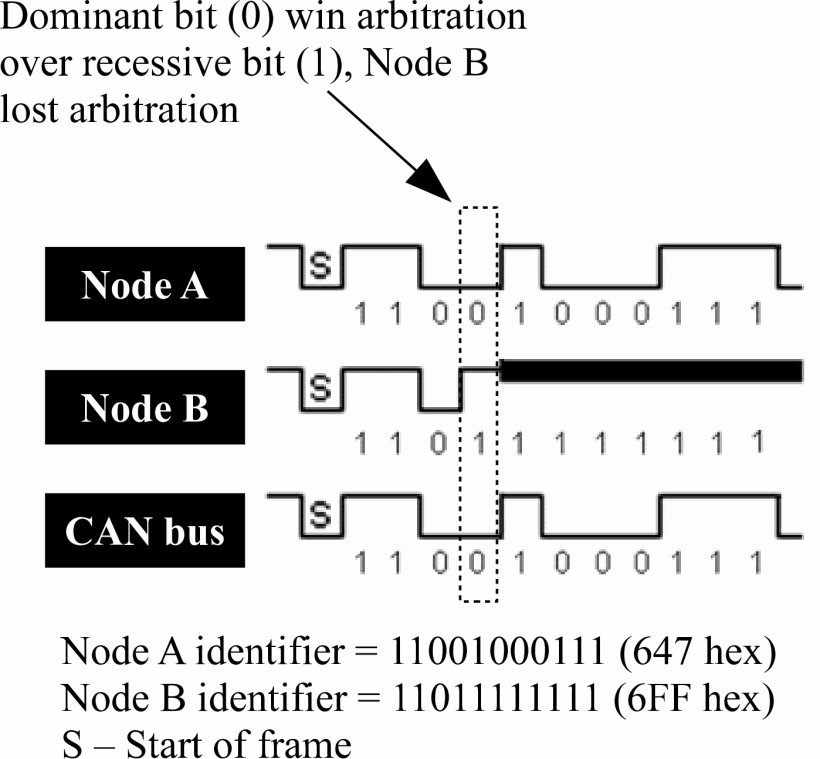
\includegraphics[width=\linewidth]{../Literatur/figures/CAN_Arbitration.png}
            \caption[
                https://ieeexplore.ieee.org/mediastore_new/IEEE/content/media/6709841/6719916/6719988/6719988-fig-2-source-large.gif
                ]{CAN-Arbitrierung}
        \end{figure}
    \end{itemize}
   
    \subsubsection{Vor- und Nachteile}
    \begin{center}
        \begin{tabular}{p{5.5cm} p{5.5cm}}
            \hline
            Vorteile & Nachteile\\
            \hline
            \hline - Kosteneffizient & - nicht Ausfallsicher\\
            \hline - einfache Konfiguration & - \\
            \hline - vielseitig & - \\
            \hline - Kompatibilität zwischen CAN generationen & - \\
            \hline
        \end{tabular}            
    \end{center}
    
\subsection{LIN-Bus}
    \subsubsection{Anwendung}
    Der LIN-Bus wurde als kostengünstige Ergänzung zum CAN-Bus entwickelt, wo dessen hohe
    Bandbreite, Resistenz gegenüber Fehler und Effizienz nicht benötigt wird. Entwickelt 
    von dem LIN-Konsortium, bestehend aus Audi, BMW, Mercedes-Benz, VW and Volvo, in den 
    späten 1990er, und veröffentlicht in 2002, sollte LIN hauptsächlich zur Kontrolle 
    simpler Mechatronischer Systeme eingesetzt werden, die keine Echtzeitkritischen Reaktion 
    erfordern. Standartisiert ist LIN nach ISO-Norm 17987.
    ~\cite{LA_Bosch_6te_auflage}\\\\
    Unter den Anwendungsgebieten befinden sich beispielhaft:
    \begin{description}
    \item[-] Ansteuerung der Fensterheber Motoren
    \item[-] Ansteuerung des Schiebedachantriebs
    \item[-] Ansteuerung des Wischermotoren
    \item[-] Auslesen von Licht-/Regensensor
    \item[-] Scheinwerferelektronik
    \item[-] Ansteuerung der Sitzmotoren
    \item[-] Gebläse/Heizelement steuerung der Klimaanlage
    \end{description}

    \subsubsection{Topologie}
    Generell wird LIN als Subbussystem/Subnetzwerk von CAN gesehen. Es besitzt dieselbe
    Busstruktur, allerdings eine weitaus geringere maximale Bandbreite von 20kBit/s, 
    die es einem LIN-Netzwerk erlauben sehr günstig in der Implementierung zu sein.
    Während andere übergeordnete Netzwerke teils über das ganze Fahrzeug verteilt tätig sind,
    befindet sich ein LIN-Netzwerk meist in einem begrenzten Bauraum (z.B. Tür). 
    ~\cite{LA_Bosch_6te_auflage}

    Ein LIN-Netzwerk nutzt das Single-Master/Multiple-Slave Struktur-Konzept, wobei der Master
    selbst als Slave fungieren kann und meist Teilnehmer in einem CAN oder FlexRay-Netzwerk ist.
    Ein Slave ist meist ein simpler Aktor, Sensor oder ein Schalter der zusätzlich die nötige Hardware 
    für eine LIN-Bus-Schnittstelle besitzt.
    ~\cite{LA_Bosch_6te_auflage}
    ~\cite{LA_LIN1}
    
    \begin{figure}
        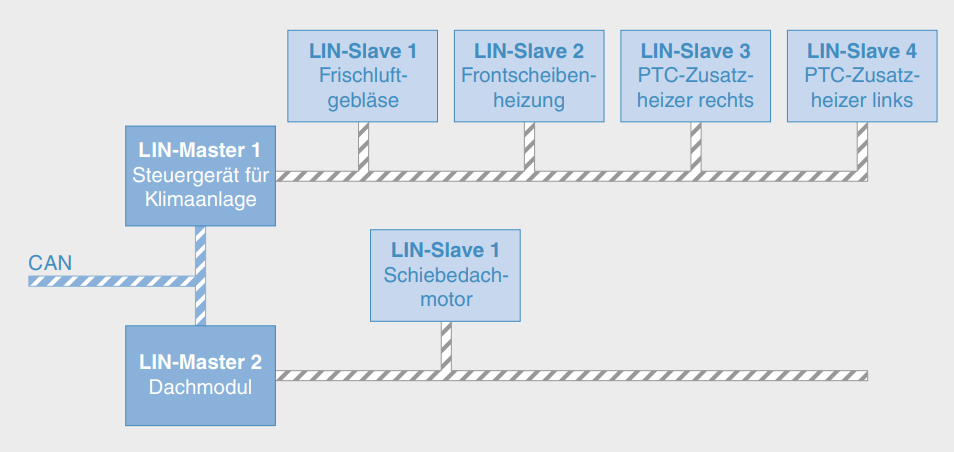
\includegraphics[width=\linewidth]{../Literatur/figures/LIN_Bus.png}
        \caption[
            https://external.dandelon.com/download/attachments/dandelon/ids/DE00247D282900209D5B0C1257814004D24BA.pdf
            ]
            {CAN/LIN-Netzwerk}
    \end{figure}

    \subsubsection{Realisierung}

    Der Buszugriff ist deterministisch über TDMA geregelt, wobei der Master das Zeitraster vorgibt.
    In einem LIN-Netzwerk werden die Nachrichten in einer Festkonfigurierten länge versendet.
    Der Master versendet Header Frames über den Bus, dieser enthält eine Botschafts-ID, um 
    den Slaves zu signalisieren welche Botschaft über den Bus gesendet werden darf. Der Slave
    der auf die Botschafts-ID konfiguriert ist sendet anschließend eine Frame Response die die 
    Daten enthält. Jeder Knoten entscheidet für sich, anhand der Botschafts-ID, ob die Daten für 
    ihn von bedeutung sind.
    Alle Botschafts-ID‘s und Nachrichtenformate müssen im vorhinein beim
    Master und den Slaves konfiguriert werden. Als Konfigurationsunterstützung sind Tools 
    erhältlich die direkt C-Code erstellen, die zur Implementierung des Masters und der Slaves
    herangezogen werden können.~\cite{LA_LIN1}\cite{LA_LDF-Tool}

    \subsubsection{Vor- und Nachteile}

    \begin{center}
        \begin{tabular}{p{5.5cm} p{5.5cm}}
            \hline
            Vorteile & Nachteile\\
            \hline
            \hline - Kosteneffizient & - geringe Bandbreite\\
            \hline - einfache Konfiguration durch Tools & - störanfällig\\
            \hline - & - viel Overhead\\
            \hline
        \end{tabular}            
    \end{center}

\subsection{FlexRay}
    \subsubsection{Anwendung}
    FlexRay entstand aus einem Konsortium von mehreren Automobil- und Microchipkonzernen bei
    dessen Konzipierung vor allem der Einsatz in Sicherheitskritischen Systemen im Vordergrund 
    stand. Dieses wurde im Jahr 2000 von BMW, DaimlerChrysler, Motorola und Philips gegründet,
    weitere Firmen wie Bosch, VW und GM traten dem Konsortium zusätzlich bei.

    FlexRay wird hauptsächlich als Bussystem für diverse X-by-Wire Systeme gesehen, die keinen 
    mechanischen Fallback besitzen, für die CAN bisher aufgrund der fehlenden Ausfall Sicherheit 
    nicht sicher eingesetzt werden konnte. Zusätzlich unterstützt FlexRay auch Bereiche wie Chassis
    Kontrolle und Komfortsysteme. 

    2006 wurde FlexRay erstmals im BMW X5 dem öffentlichen Markt zugänglich gemacht.
    ~\cite{LA_Bosch_6te_auflage}

    Auch wenn weitere OEM’s FlexRay in ihre Produktpalette mitaufgenommen haben, bleibt es
    ein Nischensystem, das sich noch nicht am breiten Markt etabliert hat. FlexRay besitzt zwar eine
    höhere Datenrate und ist Ausfallsicher, im Gegensatz zu dessen Vorgänger, CAN, erfordert 
    allerdings einen höheren Finanziellen Aufwand, sowohl in Hardware als auch in Entwicklung.
    Die höheren Kosten sind den redundanten Kanälen und der technischen Komplexität geschuldet.
    Die Gesetzliche Lage, in Deutschland~\cite{LA_StVZO38}~\cite{LA_StVZO41}
    , verbietet rein elektrische X-by-Wire Systeme. Durch 
    Einsparung der mechanischen Fallbacks, würde FlexRay preislich kompetetiver werden.
    ~\cite{LA_FR1}
    ~\cite{LA_FR2}
    ~\cite{LA_FR3}
    ~\cite{LA_FR4}
    
    2009 beendete das Konsortium die Arbeit an FlexRay mit der Spezifikation 3.0. Diese wurde
    daraufhin in den ISO-Standard 17458 überführt.\\
    Die Dokumentenlage legt nahe das FlexRay seit 2010 nicht mehr intensiv weiterentwickelt 
    wird. 
    Die Entwicklung von konkurierenden Standards wie CAN-FD ermöglichen ähnliche Datenraten.
    ~\cite{LA_FR1}
    ~\cite{LA_FR5}
    ~\cite{LA_FR6}
    
    \subsubsection{Topologie}

    FlexRay kann aufgrund der Flexibilität und der hohen Datenrate als Backbone des gesamten
    Fahrezeugnetzwerkes benutzt werden.

    \subsubsection{Realisierung}

    Damit die unterschiedlichen Anwendungsbereiche unterstützt werden können, nutzt FlexRay
    zwei Arten des Buszugriffs.
    Ein Zyklus teilt sich in zwei Segmente. Dem deterministischen Segment dessen Zugriff über
    TDMA (Time Division Multiple Access) geregelt wird und dem dynamischen Segment dessen 
    Zugriff über FTDMA (Flexible Time Division Multiple Access) geregelt wird.
    Beide Segmente sind in Zeit Slots eingeteilt, die in ihrer Länge und Anzahl frei konfigurierbar sind.\\
    \begin{itemize}
    \item{deterministisches Segment:}
    
    Jeder Zeit Slot wird einer Nachricht zugeordnet, die gesendet werden darf (ähnlich zu LIN), 
    dabei darf die Übertragungszeit nicht länger als die Zeitliche Länge des Zeit Slot sein, somit kann
    garantiert werden die Nachrichten in einer bestimmten Zeit versendet und erhaltet werden
    kann. Im deterministischen Segment werden die wichtigen und zeitlich kritischen Daten
    übertragen. \\
    
    \item{dynamisches Segment:}

    Das dynamische Segment ist ebenfalls in Zeit Slots unterteilt, denen eine Nachricht zugeordnet ist,
    die Übertragungszeit muss nicht limitiert sein, kann allerdings über Parameter eingestellt werden. 
    Die Zeitslots dienen den Steuergeräten als Startsignal, wann eine Nachricht gesendet werden darf. 
    Nachrichten werden hier nach Bedarf übertragen oder wenn das Zeitfenster im deterministischen Segment 
    nicht ausreicht.\\
    \end{itemize}

    FlexRay Netzwerke sind mit zwei Übertragungskanälen ausgestattet die über separaten Leitungen 
    verfügen. Aufgrund der Unabhängigkeit beider Kanäle ist es möglich unterschiedliche Daten über
    die Kanäle zu senden, was eine theoretische Bandbreite von bis zu 20Mbit/s ermöglicht. 
    In der Redundanten Konfiguration wird auf beiden Kanälen dieselbe Nachricht gesendet, eine 
    Ausfall Sicherheit wird somit gewährleistet.~\cite{LA_FR3}\\
    
    Die Komplexität von FlexRay stammt zusätzlich von einem hohen Freiheitsgrad in der
    Parametrisierung.\\
    In folgender Auflistung werdeen einige frei wählbaren Parameter erwähnt~\cite{LA_FR2}:
    \begin{description}
    \item[-] Zykluszeit
    \item[-] länge des deterministischen Segments
    \item[-] länge des dynamischen Segments
    \item[-] Anzahl der Zeitslot in den Segmenten
    \item[-] länge der Zeitslots
    \item[-] Redundantes/Nicht-Redundantes Versenden
    \item[-] Nachrichtenlänge im deterministischen Segment
    \end{description}

    Darüber hinaus müssen alle, in der Entwicklung eines FlexRay Netzwerkes beteiligten Hersteller, im 
    vorhinein über die finale Konfiguration des Netzwerkes Bescheid wissen, um Zykluszeiten und 
    Zeit Slot vorgaben einhalten zu kommen. Änderungen an diesen sind nur unter Schwierigkeiten möglich.


    \subsubsection{Vor- und Nachteile}
    \begin{center}
        \begin{tabular}{p{5.5cm} p{5.5cm}}
            \hline
            Vorteile & Nachteile\\
            \hline
            \hline - Ausfallsicherheit & - teurer und komplexer als alternative Bussysteme (CAN-FD, Automotive Ethernet)\\
            \hline - höhere Datenrate wie CAN &  - Bandbreite nicht ausreichend für moderne Funktionen\\
            \hline - gut anpassbar an Problemstellung & - Parametrisierung komplex\\
            \hline
        \end{tabular}            
    \end{center}

\subsection{Automotive Ethernet}
    \subsubsection{Anwendung}
    \subsubsection{Topologie}
    \subsubsection{Realisierung}
    \subsubsection{Vor- und Nachteile}

\subsection{MOST-Bus}
    \subsubsection{Anwendung}
    \subsubsection{Topologie}
    \subsubsection{Realisierung}
    \subsubsection{Vor- und Nachteile}
